\documentclass[11pt]{amsart}
\usepackage{geometry}                % See geometry.pdf to learn the layout options. There are lots.
\geometry{letterpaper}                   % ... or a4paper or a5paper or ... 
%\geometry{landscape}                % Activate for for rotated page geometry
%\usepackage[parfill]{parskip}    % Activate to begin paragraphs with an empty line rather than an indent
\usepackage{graphicx}
\usepackage{amssymb}
\usepackage{epstopdf}
\DeclareGraphicsRule{.tif}{png}{.png}{`convert #1 `dirname #1`/`basename #1 .tif`.png}

\newtheorem{Def}{Definition} %[section]
\newtheorem{Example}[Def]{Example}
\newtheorem{Prop}[Def]{Property}
\newtheorem{Lemma}[Def]{Lemma}
\newtheorem{Thm}[Def]{Theorem}
\newtheorem{Conj}[Def]{Conjecture}
\newtheorem{Cor}[Def]{Corollary}

\newcommand\bpf[1][]{\smallskip\noindent{\bf Proof#1.}\quad}
\newcommand\epf{\qed\medskip}

\newcommand\N{\mathbb N}

\title{Brief Article}
\author{The Author}
%\date{}                                           % Activate to display a given date or no date

\begin{document}

{\bf Ideas While Learning Set Theory}

These notes are not meant to be considered an academic paper,
or anything close to that. They are a collection of my personal
thoughts while learning set theory.

\section{Equivalences}

This section describes some explicitly constructed, somewhat natural 1-1 correspondences between
some collections of objects, such as sets, multi sets, lists, trees, and $\N$.

\subsection{Numbers $\leftrightarrow$ binary trees}

Choose any 1-1 correspondence $f : \N_{\ge 1} \to \N^2_{\ge 0}$.
I like to think of such a map as a counting of grid points in an array, such as this:

$$
\begin{array}{c|cccc}
 & 0 & 1 & 2 & 3 \\
 \hline
 0 & 1 & 2 & 4 & 7 \\
 1 & 3 & 5 & 8 \\
 2 & 6 & 9 \\
 3 & 10 &&& \ddots \\
\end{array}
$$

That's what Hausdorff calls ``the diagonal array.''
It's pretty easy to compute both ways.

Once you have $f = (f_1, f_2)$, then you build a binary
tree from a number $n$ recursively like this:

If $n=0$, then it's the empty tree (no root).
Otherwise, give it the left child $f_1(n)$ and
right child $f_2(n)$, keeping in mind that if
either has value 0, this means no child in that direction.
If you don't want to count the no-root tree, then start
counting at $n=1$ instead of $n=0$.

\subsection{Numbers $\leftrightarrow$ ordered $n-$ary trees}

An ordered $n-$ary tree is the natural extension of binary trees.
To be clear, binary trees are used (in my experience) most often
in a computer science context, where the left and right subtrees
are always distinguished - i.e., they are ordered. This is a bit
different from the typical math tree, where there is no intrinsic order.

The mapping is exactly the same as the binary case, except that
we must choose a 1-1 correspondence $g: \N_{\ge 1} \to \N^n_{\ge 0}$;
then the $k^\text{th}$ child of a tree numbered by $m$ will be
numbered by $g_k(m)$, where $g_k(m)$ is the  $k^\text{th}$ coordinate
of $g(m)$.

\section{Total Orders}

\subsection{A fixed-point theorem for total orders}

The following result was motivated originally by the
Banach fixed-point theorem. After proving it, I found out
about the Bourbaki-Witt (B-W) theorem, which is extremely similar,
and probably only this theorem or B-W is needed (i.e. one can be
derived easily from the other), although I haven't figured out which yet.

The notation $\sup (A)$ means $\min \{x : x \ge a \forall a \in A\}$,
which does not exist for every set $A$.

\begin{Thm}
Suppose that $X$ is totally ordered, that $\sup (A)$ exists
$\forall \text{ nonempty } A\subset X$ with an upper bound,
and that $f:X\to X$ is an
order-preserving map with $x_0 < f(x_0)$ and $f(x_1) < x_1$,
for $x_0 < x_1$. Then $\exists y \in (x_0, x_1)$ with $f(y) = y$.
\end{Thm}

\bpf
Define
$$ A = \{ y \in [x_0, x_1] : x_0 \le z \le y \implies f(z) > z \}. $$
Intuitively, $A$ is the largest convex set with left endpoint $x_0$
where $f(a) > a \forall a \in A$.

% insert set_theory_ideas1.pdf here

\centerline{
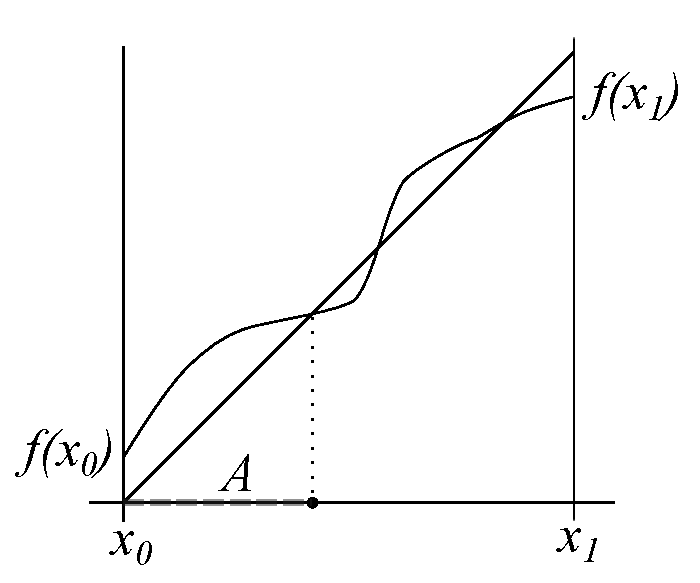
\includegraphics[width=6.0cm]{set_theory_ideas1.pdf}
}

Let $\beta = \sup (A)$, which exists since $A$ is nonempty,
having $x_0 \in A$, and has an upper bound, $x_1$.

If $\gamma = f(\beta) < \beta$, then $\gamma \in A$, but
$$ \gamma < \beta \implies f(\gamma) < f(\beta)
  \implies f(\gamma) < \gamma, $$
%$f(\gamma) = f(f(\beta)) < f(\beta) = \gamma$,
which contradicts
$f(\gamma) > \gamma$ for everything in $A$.
So $f(\beta) \ge \beta$. If $f(\beta) = \beta$, we're done,
so assume $f(\beta) > \beta$.

Suppose $w \in [x_0, x_1]$.

If $\beta < w$ and $\big(f(b) > b \,\forall\, b \in (\beta, w]\big)$,
then $w \in A$, which would contradict $w > \beta \ge A$.
So $\exists\, b_0$ with $\beta < b_0 \le w$
and $f(b_0) \le b_0$.  Then $f(\beta) < f(b_0) \le b_0 \le w$.

At this point we have both
$$ \beta < w \implies f(\beta) < w $$
and
$$ \beta > w \implies w \in A \implies f(\beta) > f(w) > w.$$

So $f(\beta) \in [x_0, x_1] \setminus \{ < \beta \} \setminus \{ > \beta \} = \{\beta\}$.
\epf

Note that $\sup (A)$ need only  exist for the specific set $A$
used in the proof, so that part of the theorem's conditions could be relaxed.

%\subsection{Matching well orders}

%This is an old idea for me, but I wanted to record it in this section.

% TODO uncomment the above and add the theorem

\section{Notes on the text of {\it Set Theory} by Felix Hausdorff}

{\bf \S 11}

Hausdorff defines the ideas of a {\it jump}, a {\it cut}, and a {\it gap} in a total order.
There's a typo in my edition where the words ``first'' and ``last'' are switched
in part of the definition.

We're talking about a total order $A$ which is partitioned into $A = P + Q$
where $P < Q$.

This table gives correct definitions for all the terms:

\bigskip
\centerline{
\begin{tabular}{c|c|c}
 & $Q$ has first & $Q$ has no first \\
 \hline
$P$ has last & jump & cut \\
$P$ has no last & cut & gap \\
\end{tabular}
}
\bigskip

{\bf \S 13}

Just before the statement of theorem III, Hausdorff is proving that all ordinal numbers are comparable,
and he states that ``The combination $\delta < \alpha, \delta < \beta$ is
also impossible, as otherwise we would have $\delta \in D$.''
It took me a few moments to figure out why that assumption lead to
$\delta\in D$, so I thought I'd write it down, even though it is really simple
once you see it. The set $D$ is defined as the intersection of $\{<\alpha\}$
and $\{<\beta\}$, so under the assumption $\delta < \alpha, \beta$, we
get $\delta\in D$ directly by the definition of $D$.

\end{document}  

% todo queue
%
% * Add a note about the "first / last" typo
% * Add a note about the infinitely many order types of type lambda
% * Add a proof for the matching well order theorem
% * Copy down a list of all the recent equivalences I know of (relevant to these notes)
% * Write up those equivalences here
%










